\section{Teststation software}

The software implemented to run the teststation essentially consists of two programs running in parallel: one taking care of the DAQ and immediate data analysis, one devoted to the slow control of the climatic chamber. 

\subsection{DAQ, Run control and test scenarios}

The ARC boards are operated with a software which is based on ARCS version 6.1~\ref{sec:arcs} and~\ref{sec:acdc}.\\
The modified ARCS version fulfills the special needs for the test station: in particular the teststation ARCS is able to perform the test on all the loaded hybrids, implements the pulse injection test and 
has been modified to interact with the slow control application in such a way tests are performed automatically once the desired environmental condition have been reached. The entire test procedure can proceed without the intervention of the operator that is only asked to load and unload the hybrids. The test scenario is given to ARCS trough a simple text file in which the sequence of operations is coded with a specific format
Beyond the high automatization, to facilitate the operator also a simple and intuitive interface has been implemented where the operator only needs to scan the bar codes of the hybrids. A screenshot of the software is shown in figure~\ref{fig:ss_arcs_teststation}.
\begin{figure}[h]
  \begin{center}
    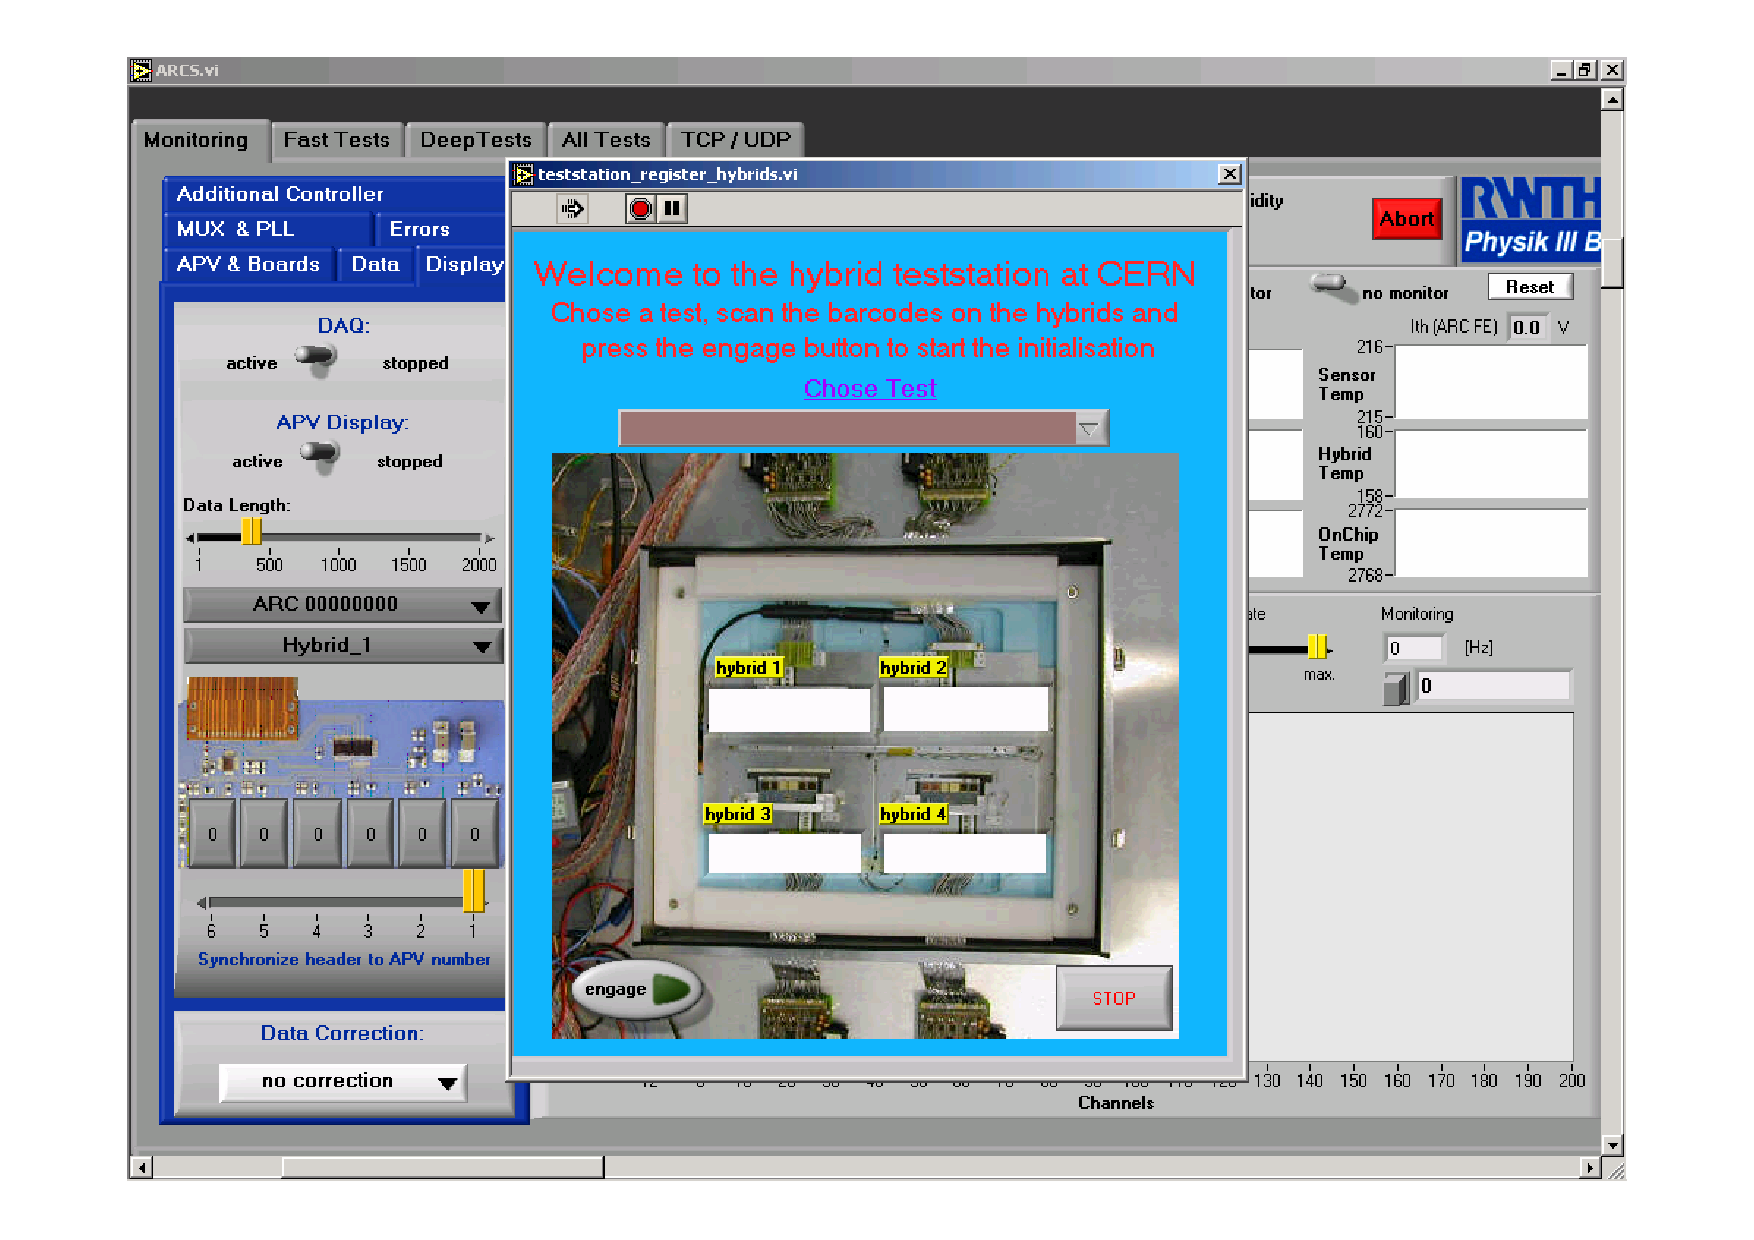
\includegraphics[width=\textwidth]{fig/ss_arcs_hybrid_test_station_mod.pdf}
%\includegraphics*[width=0.99\textwidth]{fig/cms_note.pdf}
    \caption{Screenshot of the ARCS version for the hybrid test station showing the initialization panel were only the bar codes of the hybrids have to be scanned.}
    \label{fig:ss_arcs_teststation}
  \end{center}
\end{figure}

The tests which are performed in the hybrid test station are a pedestal and noise test, a calibration pulse test at fixed timing position and the pitch adapter signal injection test.

At the end of a test, the DAQ software immediately gives to the operator feedback on the hybrid test result on the basis of the quality criteria described in~\ref{sec:}. The test results are automatically uploaded to the Tracker Construcrion Database.

\subsection{Slow control}

The main application for controlling the environmental conditions inside the hybrid test station is called ACDC. 
The software monitors and controls the temperature and the humidity of the test box and provides flags that can be queried by the ARCS system.
In this way the tests can be started when the desired temperatures are reached.
ACDC also gives alerts if any parameter leaves the range of safe operation. 
The temperature control is done regulating the current and the polarity of the peltier element. 
The difference between the actual temperature readings with respect to the required temperature are fed into a software implemented PID algorythm that returns the current value and sign (i.e. cooling or heating) that has to be driven into the peltier element through the cooli box and its built-in polarity switch.
\begin{figure}[h]
  \begin{center}
    \resizebox{\textwidth}{!}{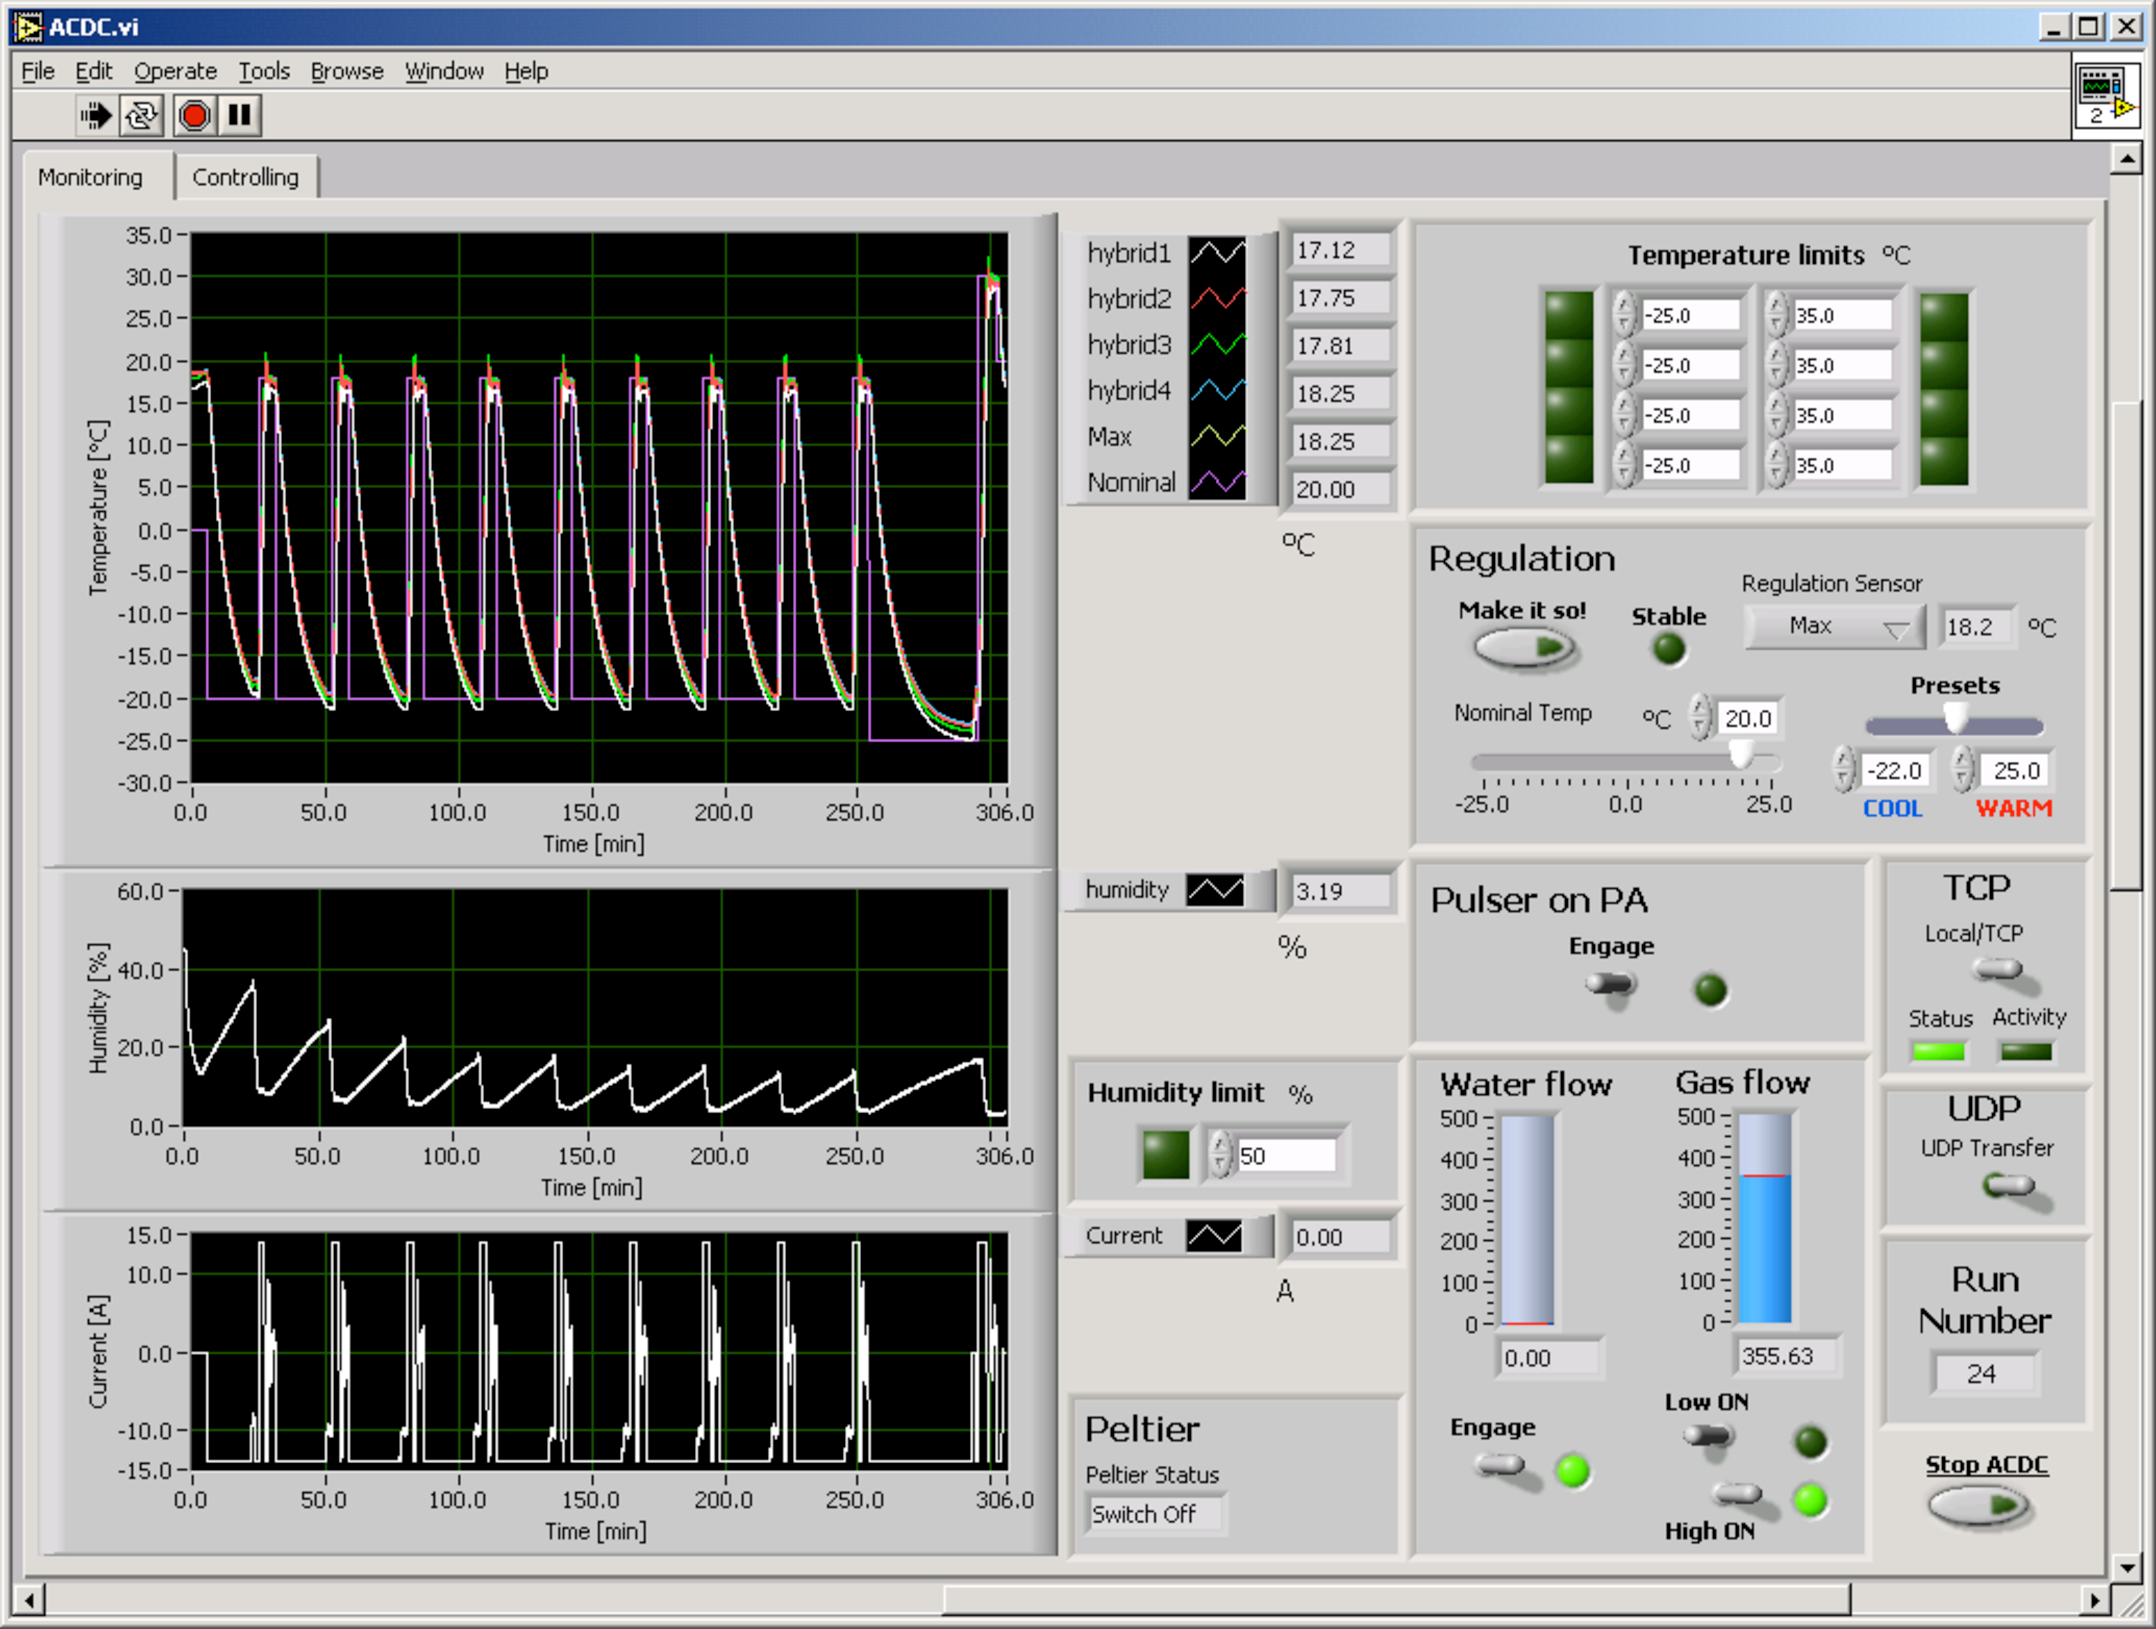
\includegraphics{fig/ACDC_screenshot.pdf}}
    \caption{Screenshot of the ACDC version for the hybrid test station.}
    \label{fig:ss_acdc_teststation}
  \end{center}
\end{figure}

